\chapter{Shape and dynamics}
\label{ch:forma}
When it's seen by naked eye, plasma sources for medical uses expel a little plume of plasma that emits radiation in a visible range, with different colours or intensity that depends on the gas composition, it's flow and intensity of applied electric field. 
However if we see this plasma at a specific time, recent studies shows that what is expelled is not a continuos flow, but the ``plume'' is formed by compact bullets with high velocities (\cite{Mericam_Bourdet_2009}, \cite{doi:10.1002/ppap.200900078}).
An example of this phenomenon is shown in figure \ref{fig:pl_bullet}, measured with the experimental apparatus that will be explained later.
\begin{figure}
 \centering
 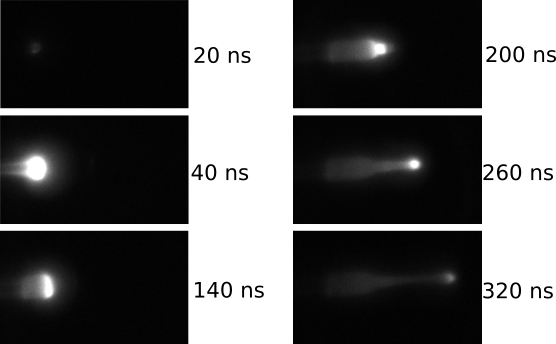
\includegraphics[width=0.8\textwidth]{Images/Shape/frames.png}
 \caption{Example of plasma bullet expulsion, as measured with our experimental setup, with an helium flow of \SI{2}{\liter/\minute}.}
 \label{fig:pl_bullet}
\end{figure}

Plasma bullets still needs to be studied in depth, we only know the basic dynamic of formation and expulsion. Some general features are that:
\begin{itemize}
 \item bullet's velocities are $> \SI{10}{\kilo\meter/\second}$;
 \item bullet formation, it's velocity and it's travel distance depend on applied tension on the electrode;
 \item frontal image of the bullet, on a plane perpendicular to it's velocity, is not a full circle but it's donut shaped, with an outer ring of higher intensity.
\end{itemize}

The scope of this experiment is to observe plasma bullets produced with our source, their shape and their velocity and how they change with different discharge conditions.

Given their typical velocities and the temperature of the plasma, bullet propagation is tought to be related to a travelling ionization front. This propagation can be studied with simplified simulation of DBD discharges, where it's reproduced the behavior of plasma bullets (\cite{doi:10.1063/1.4963115}, \cite{Breden_2012}) or the interaction between plasma and a target (\cite{doi:10.1063/1.4923345}).
%We present a simple 1D model that can reproduce the propagation of this ionization front.

\section{Experimental setup}
To visually observe dynamics of plasma formation and propagation, it is needed an acquisition setup with an high-speed camera that has little integration time, around \SI{10}{\nano\second}, and an image intensifier that permits to visualize light emitted in such a short time interval.

This is a measure where we need coincidence between discharge and frame measure so it is necessary to consider instruments and plasma source specific delays and give appropriate triggers.

Experimental setup is shown in photo \ref{fig:fotosetup} and a scheme is presented in \ref{fig:schemashape}, there are the trigger signal lines, optical acquisition pointed at source exit and measure acquisition composed by a computer and an oscilloscope. 
\begin{figure}
 \centering
 
\includegraphics[width=0.6\textwidth]{Images/Shape/acq_ottica.png}
 \caption{Photo of the experimental setup.}
 \label{fig:fotosetup}
\end{figure}

\begin{figure}
 \centering
 
\includegraphics[width=0.7\textwidth]{Images/Shape/acq_ottica.png}
 \caption{Experimental setup scheme. Function generator 1, function generator 2 and delay generator send trigger signal to camera (CCD), to source and to image intensifier (MCP), full lines in the scheme. Camera sends measured frame to a computer (PC) and from source, source's target, function generator 2 and delay are taken signals read on the oscilloscope, pointed lines in the scheme.}
 \label{fig:schemashape}
\end{figure}



\subsection{Source and optical setup}
Source head is positioned vertically and emitted light is collected from the side.
Optical apparatus is composed by a lens %specific
 coupled with a Micro Channel Plate image intensifier (MCP). An MCP works as in figure \ref{fig:MCP}: for every photon received, thanks to an high-voltage power supply, it emits many photons with little angular deviation.
\begin{figure}
 \centering
 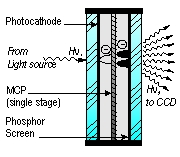
\includegraphics[width=0.4\textwidth]{Images/Shape/MCPsingle-stage.jpg}
 \caption{Micro Channel Plate image intensifier functioning.}
 \label{fig:MCP}
\end{figure}

Those photons are received by an high-speed camera \emph{Point Grey Flea} (\cite{flea}) equipped with a CCD of $\num{1024} \times \num{768}$ square pixels $\SI{4.75}{\micro\meter}$ wide. Every frame is sent to the pc where FLIR software elaborates and saves them in pgm format (\cite{pgm}).

\subsection{Source, power lines and electric signals}
It's used a source with electric features and functioning similar to those described before, with an output between $\num{3}$ and \SI{8}{\kilo\volt}, variabile changing $\Delta t$ of the trigger signal (see \ref{ch:electric}), that is always given through an optical fiber with frequency $f$. Differances are that tension is positive and not negative, because it helps formation of the plume with gasses harder to ignite (e.g. Argon), and that trigger signal is given by a generator function ($2$ in the scheme) to define discharge time respect to the trigger of other instruments.

The source is positioned vertically at a distance of \SI{42.0(1)}{\milli\meter} from optical bench, with the glass nozzle that permits to observe plasma formation inside it (external diameter \SI{8.0(1)}{\milli\meter}, internal diameter \SI{6.0(1)}{\milli\meter}), with a distance from the end of the electrode to nozzle exit of \SI{12}{\milli\meter}. At the exit the nozzle shrinks for \SI{3.0(1)}{\milli\meter}, until a diameter of \SI{5.0(1)}{\milli\meter}

Under the source is possible to put targets. Are used two different targets at different heights: conductive target and insulator target. The first one is a copper square sheet of dimensions $\SI{10}{\milli\meter} \times \SI{10}{\milli\meter} \times \SI{1}{\milli\meter}$ (used for current measures in chapter \ref{ch:electric}), the second one is a simple plastic material.


CCD camera is powered by a simple alimentator while image intensifier MCP is powered by an high-voltage supply, both are triggered by the delay generator, with different times (see next section).


On an oscilloscope are measured the trigger signal given to source head, the trigger signal given to MPC, the voltage electrode with high-voltage probe \emph{Tektronix P6015A} and the current intensity when it's used the conductive target. Current intensity measure is done measuring voltage drop on a resistance of $\SI{1}{\mega\ohm}$ with a probe $x\num{10}$.

\subsection{Trigger synchronization}
Experiment's scope is to know plasma dynamics at a specific point on voltage waveform, so it's necessary to know precisely discharge and measure times.

To compose the necessary trigger line are utilized:
\begin{itemize}
 \item function generator \emph{Or-x 310}, $1$ in figure, that sends a square wave with set amplitude, width and frequency $f$;
 \item function generator \emph{Lecroy 9210}, $2$ in figure, that sends a square wave with frequency given by the trigger, amplitude set, and variable width $\Delta t$;
 \item delay time generator \emph{Stanford DG535}, that sends square wave with set amplitude, frequency given by the voltage input and starting times given by voltage input startin time plus settable delays (4 channels).
\end{itemize}

Every intrument has it's own time that elapse between trigger signal and effective measure. The longer one is arming time for high-speed camera in the order of \si{\milli\second}, the smaller one is integration time for acquisition system, that starts from the activation of the image intensifier and span $\SI{15}{\nano\second}$.

A time line is shown in figure \ref{fig:times}, an example of signal taken with the oscilloscope is in figure \ref{fig:times_signals}. There are three relevant times defined by function and delay generators:
\begin{enumerate}
 \item $t_{0}$ is the starting time for the square wave given by \emph{Function generator 1}, with an amplitude of $\SI{5}{\volt}$ and a frequency $f$, that goes as external trigger to \emph{Function generator 2} and as voltage input to \emph{Delay generator}. From \emph{Function generator 2}, at $t_{0}$, starts the square wave that triggers discharge, with a width of $\Delta t$ that will define voltage amplitude (see chapter \ref{ch:electric}) and the same frequency $f$. From \emph{Delay generator}, at $t_{0}$, without delays, starts the trigger signal to arm the camera with the CCD.
 \item $t_{\text{DIS}}$ is the effective discharge time, when the amplitude peak starts. From trigger signal end to amplitude peak start there is a time delay given mainly by the response time of photodiode. Measuring the signals as in figure \ref{fig:times_signals}, it's possible to estimate this delay as $\SI{987.7(567)}{\nano\second}$, constant for every $f$ and $\Delta t$. Once the discharge starts, in the grey zone in figure, there are the events that we want to measure, plasma formation and propagation.
 \item $t_{\text{MIS}}$ is the measure time, when the MCP is triggered on. The delay between $t_{0}$ and $t_{\text{MIS}}$, $t_{D}$, is given by the \emph{Delay generator} with possible steps of \SI{1}{\pico\second}. Changing $t_{D}$ during measure it's possible to see plasma dynamics at different times that corresponds to different points on electrode tension waveform, as in figure \ref{fig:times_signals}.
\end{enumerate}
\begin{figure}
 \centering
 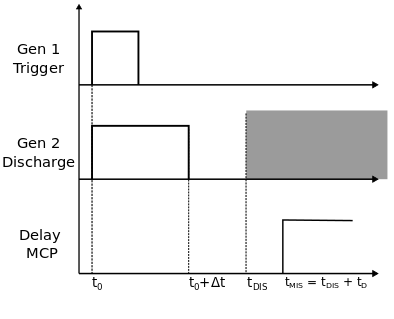
\includegraphics[width=0.6\textwidth]{Images/Shape/times.png}
 \caption{Time signal synchronization scheme: $t_{0}$ is the starting trigger time, $\Delta t$ is the opening time for plasma source (see chapter \ref{ch:electric}), $t_{\text{DIS}}$ is the starting time for the discharge and $t_{\text{MIS}}$ the starting time for the MCP i.e. the measure time}.
 \label{fig:times}
\end{figure}

\begin{figure}
 \centering
 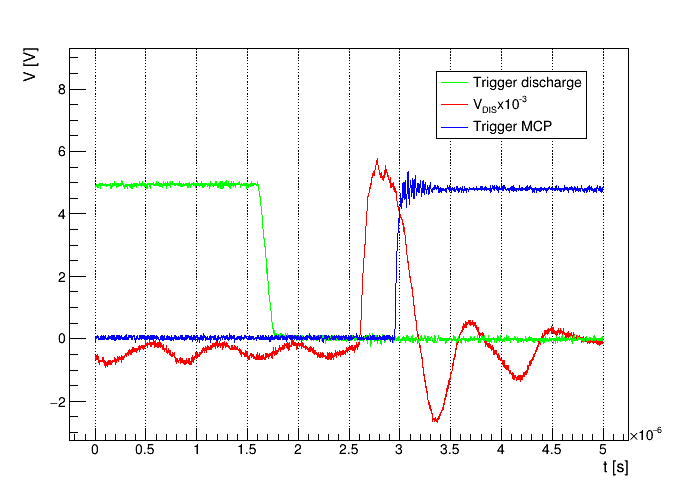
\includegraphics[width=0.6\textwidth]{Images/Shape/times_osc.png}
 \caption{Oscilloscope measure example, in green the discharge trigger, in red the electrode tension output and in blue the MCP trigger.}
 \label{fig:times_signals}
\end{figure}


Integration time for a single frame is \SI{15}{\nano\second}, so the time step between two measures has to be larger then it. For slow plasma bullets (Neon or Argon) it's used a step of \SI{50}{\nano\second}, for fast bullets (Helium) it's used a step of \SI{20}{\nano\second}.


The effective measure time have to consider slower time of the camera, larger then \SI{50}{\milli\second}. It's important to note that also with little frequencies, around \SI{50}{\hertz} (see later the minimum working frequency for different gasses), time between two pulses is \SI{20}{\milli\second}, so it is not possible to see two consecutive frames, we observe the same time in different discharges.

Changing the settings on camera acquisition software is possible to measure a signal below pixel's saturation point. One of the parameters is the \emph{Shutter time}, the opening time of the camera shutter, that if set on a value larger then the time between two signals permits to integrate between two frames.
When we work with a gas, we select an appropriate \emph{Gain} value and an appropriate \emph{Shutter time}, chosing to work measuring a single discharge frame or a multiple discharge frame.

\subsection{Different setups}
Plasma formation is influenced by many parameters such as frequency of high-voltage pulses, their rise time and maximum, gas type, gas flow, presence of a target and its features (see \cite{Mericam_Bourdet_2009}, \cite{Jarrige_2010}).

For pulse frequency we find a lower limit value, different for each ignition gas, under which there is no discharge. For frequencies higher then this value we don't expect changes (as there aren't in the electric behavior in chapter \ref{ch:electric}), so we use a single chosen value that permits plasma ignition and doesn't stress the experimental setup.
High-voltage values and gas type determine plasma bullet formation and affect its expulsion velocity. In particular, different gasses have different atomic mass and ionization energies, they will have different voltage ignition values and reactive species formed in plasma will have different velocities.
Gas flow influences how much gas there is when the ignition starts, so varying it we observe different bullets diameter and velocity.
Target influences bullet expulsion, propagation and plasma rebound signal. With a conductive target near plasma exit we will have an easier path seen by charges that propagates and, once the bullet hits the target, its observed higher luminosity going from the target to the electrode. With an insulator target we don't find the ionization channel closing on the target, but we observe charge deposition on the insulator with a shape that depends from the gas and the target.
In some setups, to help plasma ignition it's also used a conductor ring at ground potential or at floating potential, placed around source nozzle, after the electrode position.


In this study we present different setups with three different gasses, as shown in table \ref{tab:setups}.

\begin{table}
 \centering
 \begin{tabular}{cccccccc}
  \toprule
  Gas   &Setup  &$\Delta t$ &Target &Target distance    &Flow rate  &Other  &$\Delta t_D$\\
  \midrule
  \multirow{8}*{\ce{He}}    &A  &$\num{30}, \num{35}, \num{40}$ &Conductor  &\SI{24}{\milli\meter}  &\SI{2}{\liter/\minute} &-  &\SI{50}{\nano\second}\\
                            &B  &$\num{30}, \num{35}, \num{40}$ &Conductor  &\SI{32}{\milli\meter}  &\SI{2}{\liter/\minute} &-  &\SI{20}{\nano\second}\\
                            &C  &$\num{30}, \num{35}, \num{40}$ &Insulator  &\SI{24}{\milli\meter}  &\SI{2}{\liter/\minute} &-  &\SI{20}{\nano\second}\\
                            &D  &$\num{30}, \num{35}, \num{40}$ &-  &-  &\SI{2}{\liter/\minute} &-  &\SI{20}{\nano\second}\\
                            &E  &$\num{35}$ &-  &-  &\SI{2}{\liter/\minute} &Ground ring  &\SI{20}{\nano\second}\\
                            &F  &$\num{35}$ &-  &-  &\SI{1}{\liter/\minute} &-  &\SI{20}{\nano\second}\\
                            &G  &$\num{35}$ &-  &-  &\SI{3}{\liter/\minute} &-  &\SI{20}{\nano\second}\\
                            &H  &$\num{35}$ &-  &-  &\SI{4}{\liter/\minute} &-  &\SI{20}{\nano\second}\\
  \midrule
  \multirow{5}*{\ce{Ne}}    &A  &$\num{20}, \num{25}, \num{30}$ &Conductor  &\SI{24}{\milli\meter}  &\SI{2}{\liter/\minute} &-  &\SI{50}{\nano\second}\\
                            &B  &$\num{20}, \num{25}, \num{30}$ &Conductor  &\SI{32}{\milli\meter}  &\SI{2}{\liter/\minute} &-  &\SI{50}{\nano\second}\\
                            &C  &$\num{20}, \num{25}, \num{30}$ &Insulator  &\SI{24}{\milli\meter}  &\SI{2}{\liter/\minute} &-  &\SI{50}{\nano\second}\\
                            &D  &$\num{20}, \num{25}, \num{30}$ &-  &-  &\SI{2}{\liter/\minute} &-  &\SI{50}{\nano\second}\\
                            &E  &$\num{30}$ &-  &-  &\SI{2}{\liter/\minute} &Ground ring  &\SI{50}{\nano\second}\\
  \midrule
  \multirow{6}*{\ce{Ar}}    &A  &$\num{35}$ &-  &-  &\SI{2}{\liter/\minute} &Ground ring  &\SI{50}{\nano\second}\\
                            &B  &$\num{35}$ &-  &\SI{32}{\milli\meter}  &\SI{2}{\liter/\minute} &-  &\SI{20}{\nano\second}\\
                            &C  &$\num{35}$ &-  &-  &\SI{2}{\liter/\minute} &Floating ring  &\SI{50}{\nano\second}\\
                            &D  &$\num{35}$ &Conductor  &\SI{20}{\milli\meter}  &\SI{2}{\liter/\minute} &Ground ring  &\SI{50}{\nano\second}\\
                            &E  &$\num{35}$ &Conductor  &\SI{20}{\milli\meter}  &\SI{2}{\liter/\minute} &-  &\SI{50}{\nano\second}\\
                            &F  &$\num{35}$ &-  &-  &\SI{2}{\liter/\minute} &-  &\SI{50}{\nano\second}\\
                            &G  &$\num{35}$ &Conductor  &\SI{32}{\milli\meter}  &\SI{2}{\liter/\minute} &-  &\SI{50}{\nano\second}\\
  \bottomrule
 \end{tabular}
 \caption{Description of measure setups. In first column there is the gas; second column is the setup name; third column is voltage pulse time width, expressed as percentage of a square trigger \SI{10}{\micro\second} long; four and fifth columns are target information, where it's used a target; sixth column is used gas flow; seventh column are other informations, i.e. if it's used the conductor ring explained before; eight column is the time step between two different frames.}
 \label{tab:setups}
\end{table}


\subsection{Frame analysis and calibration}
Once a measure setup is chosen, $t_D$ is set around the start of the discharge, we measure the oscilloscope waveform for every channel (setup as explained before), and from them we save $5$ frames for every $t_D$ varying it with steps of $\Delta t_D$. Measures are taken until the end of the main tension peaks and the camera doesn't see anything.


From oscilloscope waveforms we can extrapolate the measure time from the start of the discharge and tension value at measure time. When there is the conductive target it's also possible to see current intensity and it's peak time.


Frame analysis is done converting the pgm files in 2-dimensional histograms, using \emph{TH2} class written in \emph{ROOT} libraries (see \cite{ROOT:TH2}).
We are interested in plasma bullet formation and it's expulsion, but also in other fenomenological behavior that is observed during measures.

For plasma bullet we take the mean for every pixel between the five frames taken, from then it's isolated the plasma bullet as the collection of pixels with maximum intensity in the frame. From this image we extrapolate the position of the bullet with the coordinates of it's luminosity barycenter on the plane seen by camera, called x-y in the analysis.
Once established the center, we can find it's contour as the points were luminosity goes under a certain percentage of the maximum, from that we estimate it's dimensions along x and y axis and it's average luminosity.
With barycenter coordinates it's possible to compute their velocity using a finite differance formula (that takes into consideration possible different time steps, see \cite{Bhadauria}).


Actual dimensions on a frame are found with a calibration with a known target: it is used a plate with $4$ holes, diameter of \SI{1.0(1)}{\milli\meter} at the vertice of a square with an edge lenght of \SI{10.0(1)}{\milli\meter}, positioned at plasma exit (source is off) and illuminated from behind with a torch.
Acquiring a frame of this setup it's possible to extrapolate pixel's distance that corresponds to \SI{10}{\milli\meter} for every square edge, average them, and calculate pixel's width in our frames, resulting a value of $d_{pix} = \SI{0.172(2)}{\milli\meter}$.

\section{Helium flow}
We start the presentation of measures with helium, as it is commonly used for medical applications of plasma.
Helium it's an element with standard atomic weight of $\num{4.002}$, 1st ionization energy of \SI{24.587}{\electronvolt} and 2nd ionization energy of \SI{54.418}{\electronvolt}.
It's easy to produce helium plasma, when it's ignited it emits radiation with principal wavelenghts in violet and orange ($\lambda = \num{388.86}$ and \SI{587.56}{\nano\meter}), resulting in a purple plume at naked eye.
Principal downside of helium gasses it's that they are expensive.


In our experiment we produce helium plasma with pulse frequency $f = \SI{5}{\kilo\hertz}$ and $\Delta t = \num{3}$, $\num{3.5}$ and \SI{4}{\micro\second}, as explained in table \ref{tab:setups}.
Delays are setted to take a single frame during every acquisition, for every measure we take $5$ frames and average them.


First we present a tipical discharge without target, after is shown how the behavior changes varying parameters and then it's discussed how a target influences bullet propagation.

\subsection{Plasma bullet description}
We use as example bullet the setup D with $\Delta t = \SI{3.5}{\micro\second}$, i.e. absence of a target and gas flow of \SI{2}{\liter/\minute}.


It's possible to divide the phenomenon that we want to observe in four phases, as presented in figure \ref{fig:bullet_es}: bullet formation, bullet displacement inside the nozzle, bullet expulsion and bullet propagation outside the nozzle, in air. It's important to remember that time values goes from the start of the voltage peak, extrapolated from oscilloscope measures.
When the voltage goes over a definite value, we observe a rapid increase in luminosity around the electrode that it's interpreted as plasma formation. From there, in a time of $\sim \SI{50}{\nano\second}$ the plasma modifies it'shape and becames what we call the bullet: a zone with high luminosity confined in space. The bullet then moves in the exit direction and it's expelled always with a well defined front. In air we see the round shaped bullet propagation, until it reaches a maximum travel distance and then luminosity decreases rapidly, until we see nothing more. In these measure conditions we see again plasma formation in correspondence of the negative tension peak, but it is  a rapid process without propagation.
\begin{figure}
 \centering
 \subfloat[\SI{140.93}{\nano\second}]{
    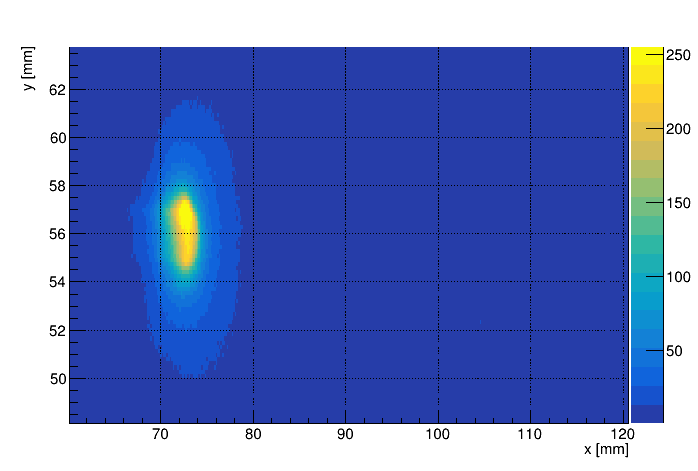
\includegraphics[width=0.48\textwidth]{Images/Shape/elio_d035_es1.png}
 }
 \hfill
 \subfloat[\SI{240.93}{\nano\second}]{
    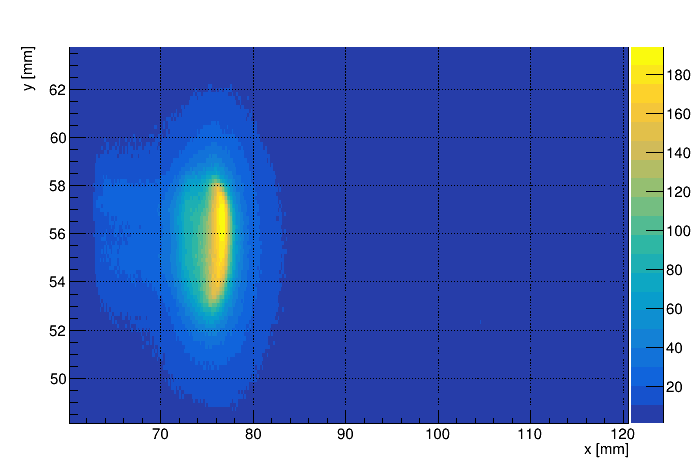
\includegraphics[width=0.48\textwidth]{Images/Shape/elio_d035_es2.png}
 }
 
 \subfloat[\SI{400.93}{\nano\second}]{
    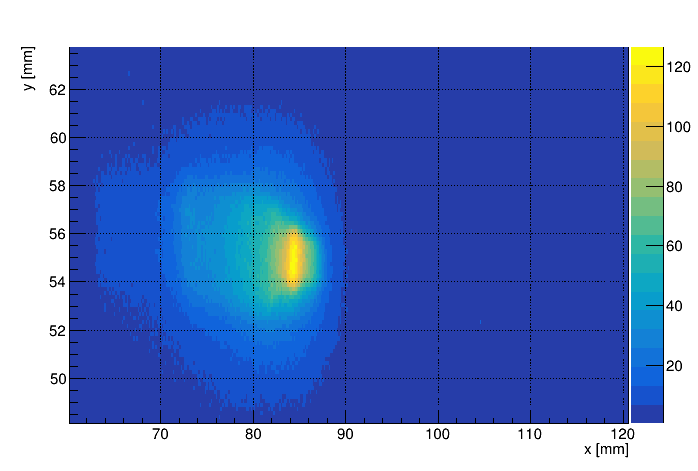
\includegraphics[width=0.48\textwidth]{Images/Shape/elio_d035_es3.png}
 }
 \hfill
 \subfloat[\SI{460.93}{\nano\second}]{
    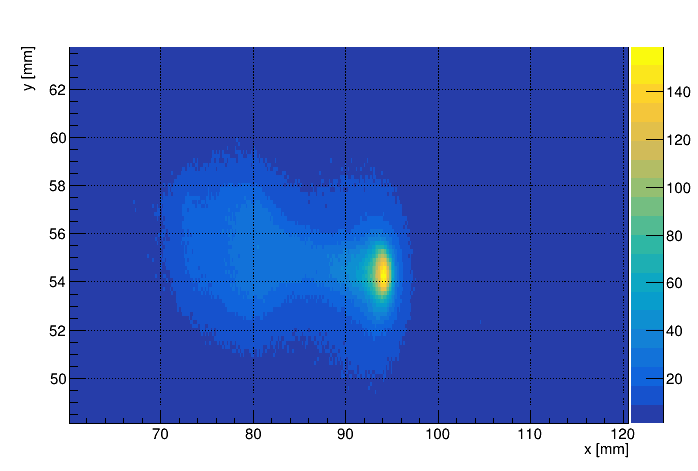
\includegraphics[width=0.48\textwidth]{Images/Shape/elio_d035_es4.png}
 }
 \caption{Four phases of plasma dynamics: bullet formation (a), bullet displacement inside the nozzle (b), bullet expulsion (c) and bullet propagation outside the nozzle (d). Time intervals are calculated from the start of the voltage peak.}
 \label{fig:bullet_es}
\end{figure}


\paragraph{Electrode voltage and bullet intensity}
The time interval in wich we see the bullet can be defined as where we can see a definite zone with mean luminosity higher then the background. The starting time is given by voltage reaching a certain value, when we see bullet formation, and the bullet expires when it's luminosity decreases.

In figure \ref{fig:elio_d035_I} are presented the mean intensity of the plume during the motion and the zoom on the intersted time interval for voltage measure. Plasma formation is observed around \SI{120.93}{\nano\second} after peak start, at a tension value of \SI{5710.00(28550)}{\volt}. %while maximum peak value is \SI{6588.80(32944)}{\volt} at time \SI{260.93}{\nano\second}.
As we can see, luminosity is higher during plasma formation around the electrode and it decrease very little during all the propagation, even after the expulsion in air (pointed line on the graph). After a time of \SI{440}{\nano\second} the bullet luminosity decreases rapidly and it disperses in the air.
\begin{figure}
 \centering
 \subfloat[Zoom on voltage waveform.]{
    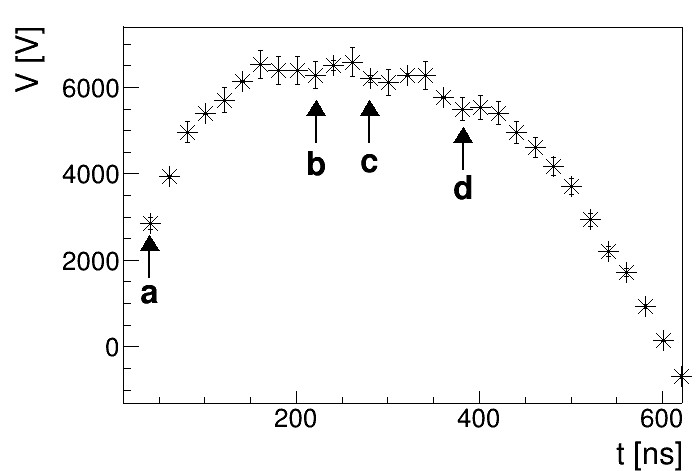
\includegraphics[width=0.48\textwidth]{Images/Shape/elio_d035_V.png}
 }
 \hfill
 \subfloat[Mean intensity of plasma bullet.]{
    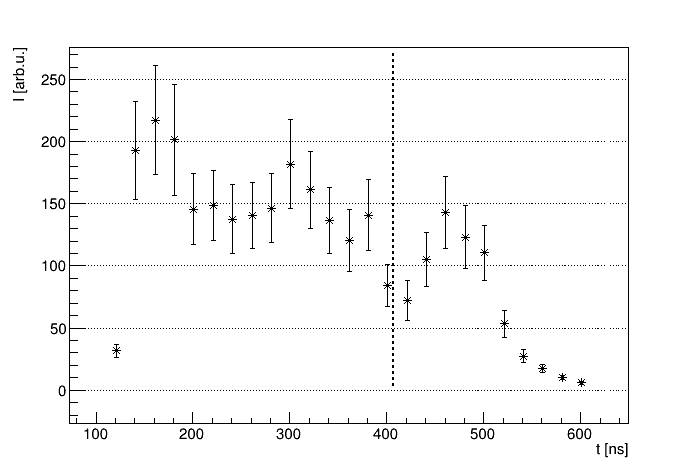
\includegraphics[width=0.48\textwidth]{Images/Shape/elio_d035_Im.png}
 }
 \caption{Voltage waveform and intensity of the bullet versus time. Time zero is the start of the voltage peak, ending time is taken as the time where intensity reaches background value. The pointed line in intensity graph indicates the end of the nozzle.}
 \label{fig:elio_d035_I}
\end{figure}

\paragraph{Barycenter coordinates and direction}
The motion of the bullet on observing plane can be extrapolated from it's barycenter coordinates.

In figure \ref{fig:elio_d035_bary} there are the two coordinates versus time.
Coordinate x, along the axis of the source (of the electrode and the nozzle) is more relevant to observe bullet expulsion. We see as plasma forms around position $\SI{73}{\milli\meter}$ and the nozzle ends at $\SI{85}{\milli\meter}$, compatible with the distance electrode-nozzle exit described before. After plasma formation we can see bullet displacement in the nozzle with a certain velocity, until it reaches the exit and propagates in the air more rapidly. The bullet travels until it reaches a maximum x, covering a distance of \SI{26.08(2)}{\milli\meter} from the electrode. It seems that the bullet stops while it's luminosity decreases.

Coordinate y it's relevant to show bullet direction, as we can see, it moves in a space interval of \SI{2}{\milli\meter}. The bullet forms over the electrode, then, when it enlarges to cover all the nozzle diameter, lowers it's barycenter with a constant slope, even after the expulsion. Once the bullet starts to decrease in luminosity, it stops its motion also on the y direction.
\begin{figure}
 \centering
 \subfloat[]{
    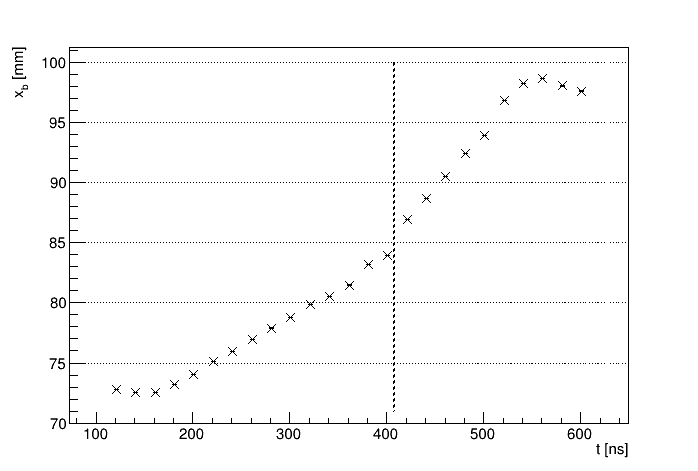
\includegraphics[width=0.48\textwidth]{Images/Shape/elio_d035_xb.png}
 }
 \hfill
 \subfloat[]{
    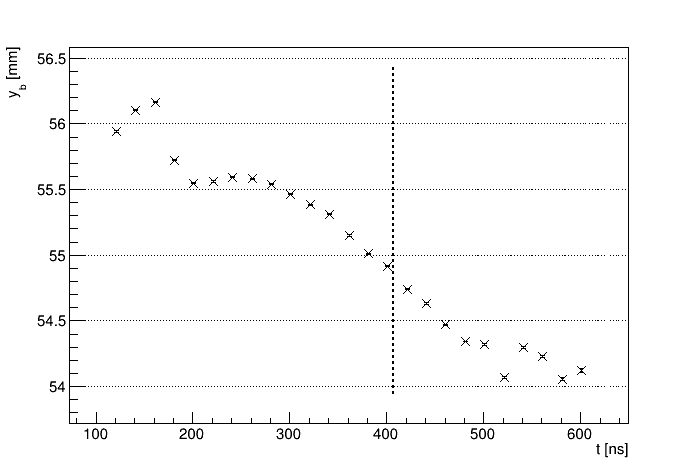
\includegraphics[width=0.48\textwidth]{Images/Shape/elio_d035_yb.png}
 }
 \caption{Barycenter coordinates of the bullet. Pointed lines indicate the end of the nozzle.}
 \label{fig:elio_d035_I}
\end{figure}

Lowering of the baricenter in the y direction it's explainable by a tilt in the source, that is not perfectly perpendicular to the optical bench, if we consider the entire dimension of the bullet in the y direction, with it's upper and lower limits. In figure \ref{fig:elio_d035_diry} are shown y maximum, minimum and baricenter of the bullet, in function of the x brycenter coordinate and can be seen how the entire figure points downward (to the side turning the image). Inside the nozzle we can take y maximum as a value that defines the contour of the nozzle, with a fit as in figure we find a value of \SI{3.39(10)}{\degree}. Outside the nozzle we find that the barycenter direction is pointed \SI{3.71(4)}{\degree} downward, a little higher then the direction of the nozzle. The values are almost compatible with each other, so it seems to suggest that tilting the source it's possible to direct the bullet even after it's propagation in air.
\begin{figure}
 \centering
 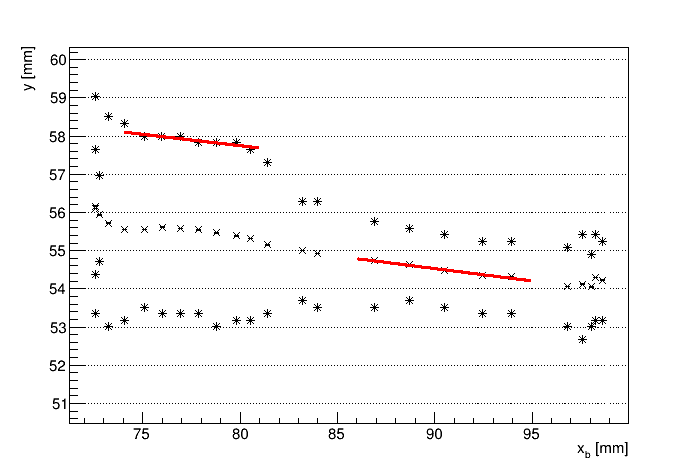
\includegraphics[width=0.6\textwidth]{Images/Shape/elio_d035_incl.png}
\end{figure}


\paragraph{Bullet dimensions}
Once we define the contour of the bullet, it's simple to take it's dimensions along the two directions.

In figure \ref{fig:elio_d035_dim} are presented width and height of the bullet.
In the x direction, the bullet presents constant diameter until it approaches nozzle exit, where it enlarges a little to reach the exit. In the air the bullet mantaines its dimension, with values a little lower then inside the nozzle, but compatible within the error. When it stops it seems to have greater diameter, but the measure loses significance as the bullet fades in the air and it can be confused with the background.
In y direction we find a constant value of \SI{4.65(20)}{\milli\meter} during propagation in the nozzle, as expected because the bullet covers all the nozzle area, a little lower then its diameter due to glass refraction effects. Once the nozzle shrinks, the bullet diminish it's diameter and maintains a constant value of \SI{2.07(20)}{\milli\meter} during all the propagation in air, until it stops.
\begin{figure}
 \centering
 \subfloat[]{
    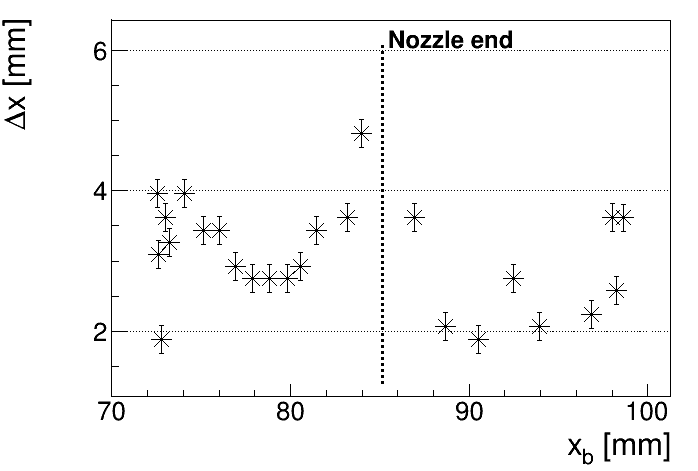
\includegraphics[width=0.48\textwidth]{Images/Shape/elio_d035_dx.png}
 }
 \hfill
 \subfloat[]{
    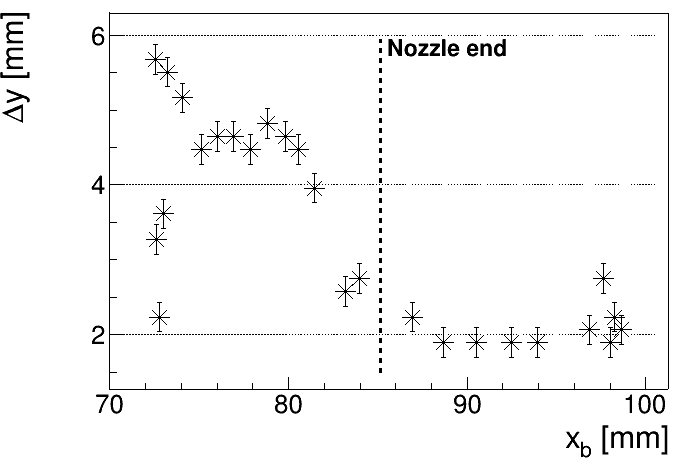
\includegraphics[width=0.48\textwidth]{Images/Shape/elio_d035_dy.png}
 }
 \caption{Dimensions of the bullet. Pointed lines indicate the end of the nozzle.}
 \label{fig:elio_d035_I}
\end{figure}


\paragraph{Bullet velocity}
From barycenter graphs we see as bullet motion has a definite velocity during described phases.
Fitting the graph with a line during the displacement phase inside the nozzle, as in figure \ref{fig:elio_d035_vx}, we find that it moves with a speed of $v_{\text{disp}} = \SI{46.48(20)}{\kilo\meter/\second}$. Once it exits the nozzle it speeds up, until a value of $v_{\text{prop}} = \SI{95.16(60)}{\kilo\meter/\second}$.


With a 3 point finite differance formula we can estimate it's velocity point by point (excluding the first and the last), finding the values shown in figure \ref{fig:elio_d035_vx}. From those values we can average velocities during the two motion phases, finding compatible mean value respect the linear fit: $v_{\text{disp}} = \SI{48.23(103)}{\kilo\meter/\second}$ and $v_{\text{prop}} = \SI{95.16(182)}{\kilo\meter/\second}$.
\begin{figure}
 \centering
 \subfloat[Fit of x barycenter.]{
    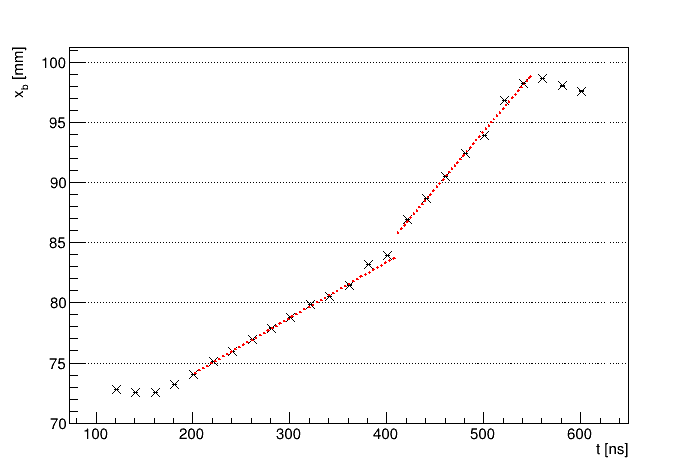
\includegraphics[width=0.48\textwidth]{Images/Shape/elio_d035_xb_fitv.png}
 }
 \hfill
 \subfloat[Velocities in x direction.]{
    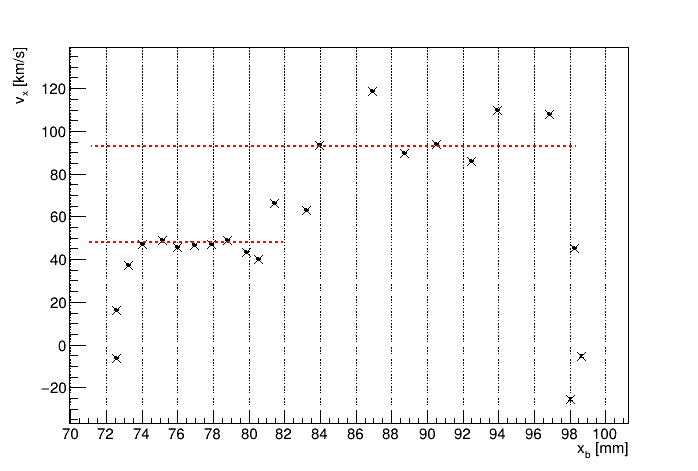
\includegraphics[width=0.48\textwidth]{Images/Shape/elio_d035_vx_fitv.png}
 }
 \caption{Velocity of the bullet in x direction. Pointed lines indicate the end of the nozzle, red lines calculated values during displacement and propagation phases.}
 \label{fig:elio_d035_vx}
\end{figure}

It's interesting to point out that those velocities are much higher then the average velocity of the neutral gas, that for a flow of \SI{2}{\liter/\minute} is of \SI{12}{\meter\second}.

\subsection{Voltage influence}
With an higher $\Delta t$ we can reach higher voltage peak values (see chapter \ref{ch:electric}), so we will have higher electron energies. With more energy we expect that the bullet will reach furter distances, with higher velocity. In figure \ref{fig:elio_d} and table \ref{tab:elio_d} are presented the results of the analysis.

The discharge starts always in the same voltage interval, around \SI{5.7}{\kilo\volt}. We observe a higher luminosity with higher tensions, but it decreases always in a time interval around \SI{100}{\nano\second} once it exits the nozzle (figure \ref{fig:elio_d} (a)).

The plot for the barycenter coordinates (figure \ref{fig:elio_d} (b) - (c)) shows how with higher voltage the bullet reaches further distances ($x_{\text{dist}}$ and $y_{\text{dist}}$ in table). For the lower voltage peak it seems that the bullet doesn't propagate in air, as it stops right after nozzle exit.

Dimensions of the bullet (figure \ref{fig:elio_d} (d) - (e)) are not influenced by voltage value, as we can see they have the exact same behavior, around the same values, for every opening time. A notable differance it's in the y diameter inside the nozzle, where for higher tension we have a slightly larger value. As mentioned before here we have refraction effects due to the glass nozzle, different for those measures due to the higher luminosity.

Velocity values (figure \ref{fig:elio_d} (f)) show how the bullet behavior is solid during the propagation inside the nozzle and becames more erratic once it exits. As mentioned before, for the lowest opening time we have lower velocities and a rapid drop after contact with air, in this configuration it's not possible to find a propagation velocity. For higher opening times we find the same behavior, with a proportionality between peak voltage value and velocities: if before we found a stable motion with $v_{\text{prop}} = \SI{92.93(6)}{\kilo\meter/\second}$, with higher tension it reaches $v_{\text{prop}} = \SI{149.47(9)}{\kilo\meter/\second}$.

\begin{figure}
 \centering
 \subfloat[Mean luminosity.]{
    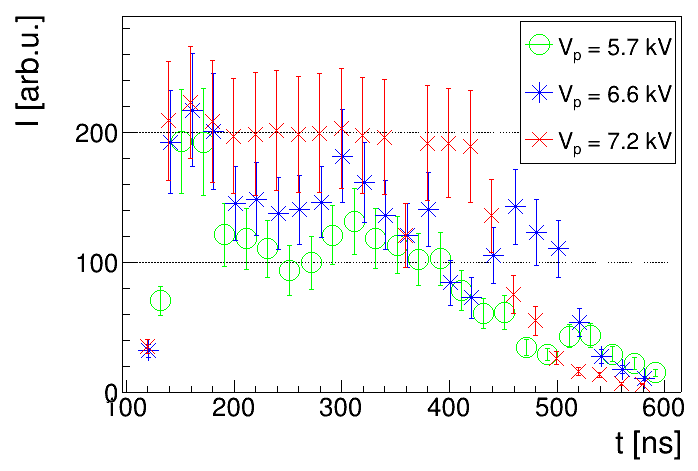
\includegraphics[width=0.48\textwidth]{Images/Shape/elio_d_Im.png}
 }
 \hfill
 \subfloat[x barycenter.]{
    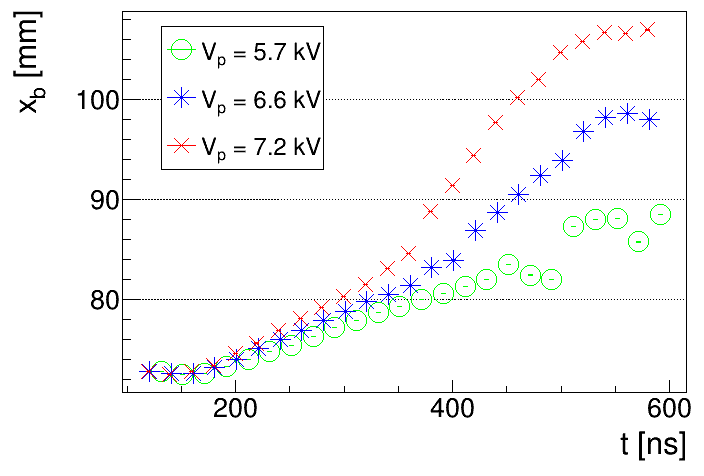
\includegraphics[width=0.48\textwidth]{Images/Shape/elio_d_xb.png}
 }
 \subfloat[y barycenter.]{
    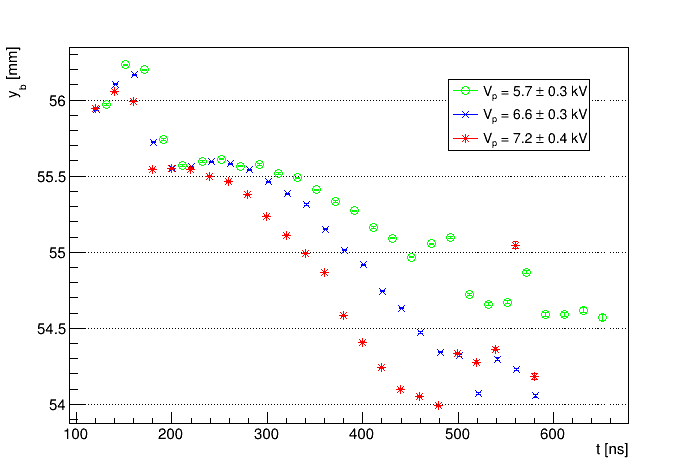
\includegraphics[width=0.48\textwidth]{Images/Shape/elio_d_yb.png}
 }
 \hfill
 \subfloat[x diameter.]{
    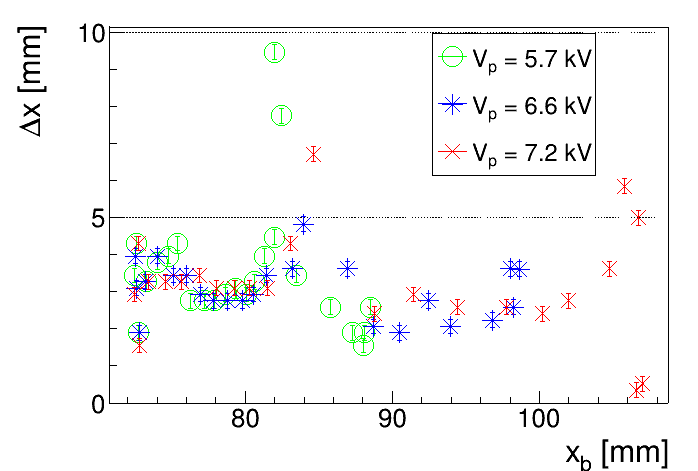
\includegraphics[width=0.48\textwidth]{Images/Shape/elio_d_dx.png}
 }
 \subfloat[y diameter.]{
    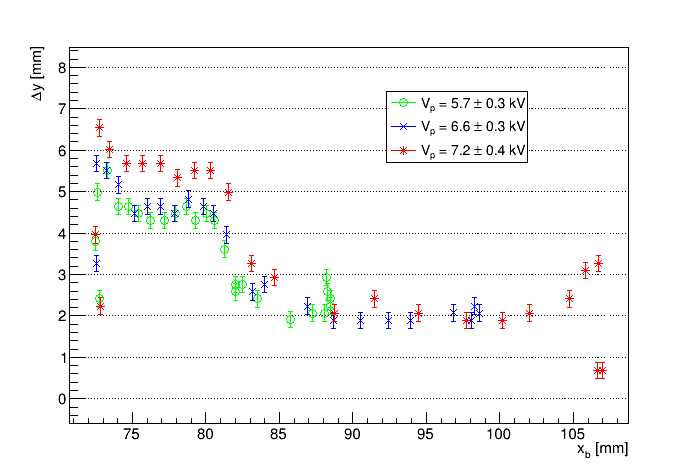
\includegraphics[width=0.48\textwidth]{Images/Shape/elio_d_dy.png}
 }
 \hfill
 \subfloat[x velocity.]{
    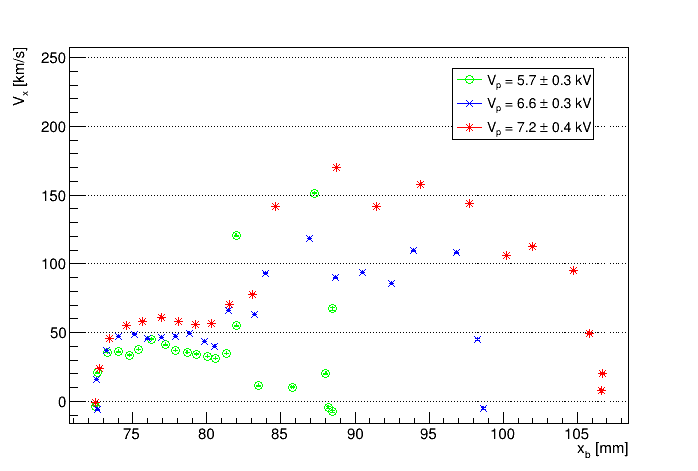
\includegraphics[width=0.48\textwidth]{Images/Shape/elio_d_vx.png}
 }
 \caption{Results of the analysis for setup d (helium flow of \SI{2}{\liter/\minute} without target), with different peak voltage values.}
 \label{fig:elio_d}
\end{figure}

\begin{table}
 \centering
 \begin{tabular}{ccccccc}
 \toprule
 $V_{p}$ [kV]    &$t_{0}$ [ns] &$V_{0}$ [kV]    &$x_{\text{dist}}$ [mm]   &$y_{\text{dist}}$ [mm]   &$v_{\text{disp}}$ [km/s]   &$v_{\text{prop}}$ [km/s]\\
 \midrule
 \num{5.66(30)}  &\num{131.5}  &\num{5.55(28)}    &\num{15.99(1)} &\num{1.66(2)}  &\num{37.72(4)} &-\\
 \num{6.59(33)}  &\num{120.9}  &\num{5.71(29)}    &\num{26.08(2)} &\num{1.92(4)}  &\num{46.48(2)} &\num{95.16(6)}\\
 \num{7.22(36)}  &\num{119.5}  &\num{6.01(30)}    &\num{34.55(5)} &\num{2.07(1)}  &\num{59.80(3)} &\num{149.47(9)}\\
 \bottomrule
 \end{tabular}
 \caption{Result of the analysis with different voltage peak values for the pulse. $V_{p}$ is the peak value for the pulse, $t_{0}$ bullet formation time, $V_{0}$ bullet formation tension, $x_{\text{dist}}$ and $y_{\text{dist}}$ are the highest distances reached by the bullet from electrode position, $v_{\text{disp}}$ is the velocity in x direction reached inside the nozzle, $v_{\text{prop}}$ is the velocity of propagation in air in x direction.}
 \label{tab:elio_d}
\end{table}


\subsection{Flow influence}
As said before, neutral gas velocity is very little in comparision of the ionization front velocity of the bullet, we expect that changes in the gas flow will have an effect on the quantity of helium present in the nozzle more then on the energy of the atoms and electrons. We try four different flows with the same peak voltage, in figure \ref{fig:elio_d} and table \ref{tab:elio_d} are presented the results of the analysis.

Also for this parameter, the discharge starts always in the same voltage interval, around \SI{5.7}{\kilo\volt}. For gas flows of $\num{1}$ and \SI{2}{\liter/\minute} bullet luminosity decreases in a time interval around \SI{100}{\nano\second} once it exits the nozzle, for higher flows it has a luminosity clearly stronger then background for a longer time interval, around \SI{200}{\nano\second} (figure \ref{fig:elio_035} (a)).

From the barycenter coordinates (figure \ref{fig:elio_d} (b) - (c)) we see as more gas flow seems to be correlated with lower mobility of the bullet: we have shorter distances with higher flows. For maximum tried flow, even if bullet luminosity is more then the background, the bullet travels a very little distance from the exit of the nozzle and it's barycenter remains almost fixed in space.

Dimensions of the bullet (figure \ref{fig:elio_d} (d) - (e)) are not very  influenced by gas flow, but we can see little inverse proportionality. For stronger flows we have always littler diameters inside the nozzle, in both directions.

Velocities shows how the bullet behavior changes also inside the nozzle varying gas flow (figure \ref{fig:elio_d} (f)). With little flow, we find a costant displacement velocity in the nozzle, while with more flow the bullet slows down when moving (as shown in \cite{Jarrige_2010}), with a decrease in velocity of \SI{7.58(4)}{\kilo\meter/\second/\milli\meter}.
Once the bullet exits the nozzle, we see how it almost stops when there is high flow, while it shows the same behavior if flow is under \SI{3}{\liter/\minute} and it has maximum velocity for the lowest gas flow, maintaining it for longer time.


Can be concluded that with higher flow we have bullet with longer lifetime and littler mobility, reaching lesser distances with lesser velocity.


\begin{figure}
 \centering
 \subfloat[Mean luminosity.]{
    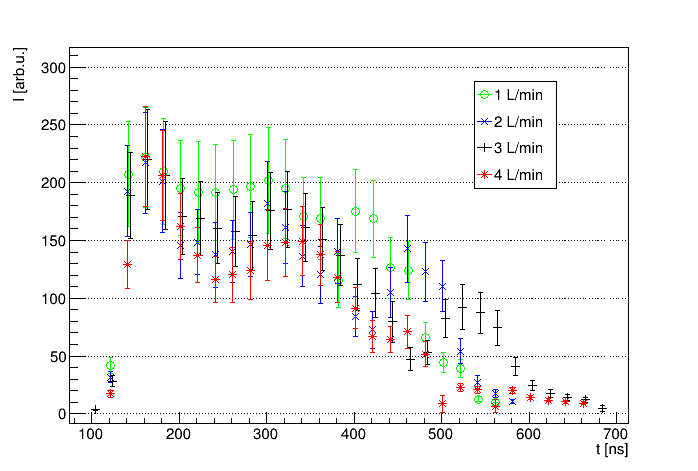
\includegraphics[width=0.48\textwidth]{Images/Shape/elio_035_Im.png}
 }
 \hfill
 \subfloat[x barycenter.]{
    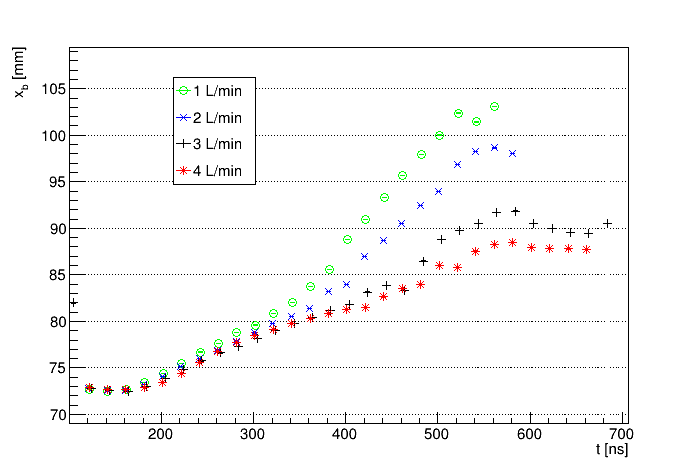
\includegraphics[width=0.48\textwidth]{Images/Shape/elio_035_xb.png}
 }
 \subfloat[y barycenter.]{
    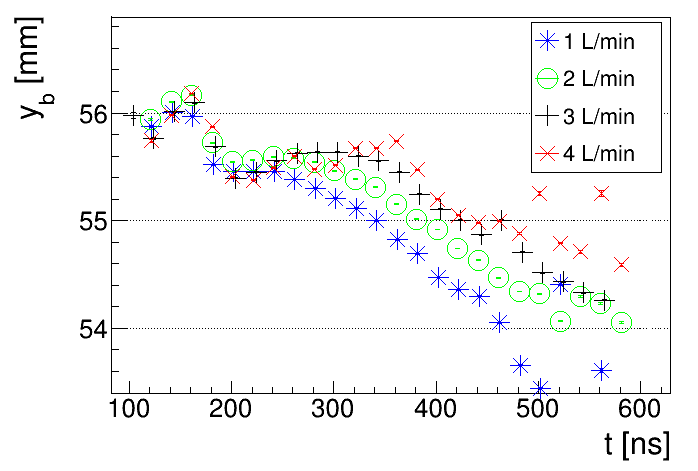
\includegraphics[width=0.48\textwidth]{Images/Shape/elio_035_yb.png}
 }
 \hfill
 \subfloat[x diameter.]{
    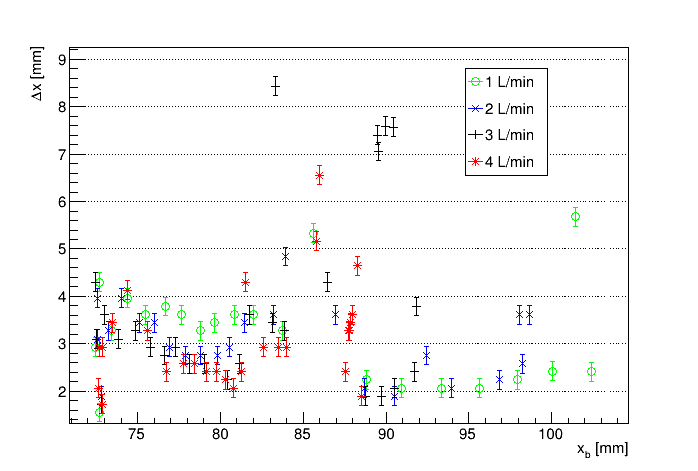
\includegraphics[width=0.48\textwidth]{Images/Shape/elio_035_dx.png}
 }
 \subfloat[y diameter.]{
    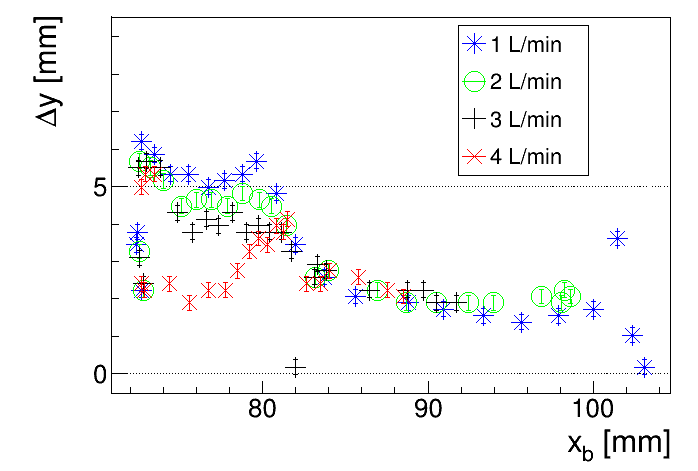
\includegraphics[width=0.48\textwidth]{Images/Shape/elio_035_dy.png}
 }
 \hfill
 \subfloat[x velocity.]{
    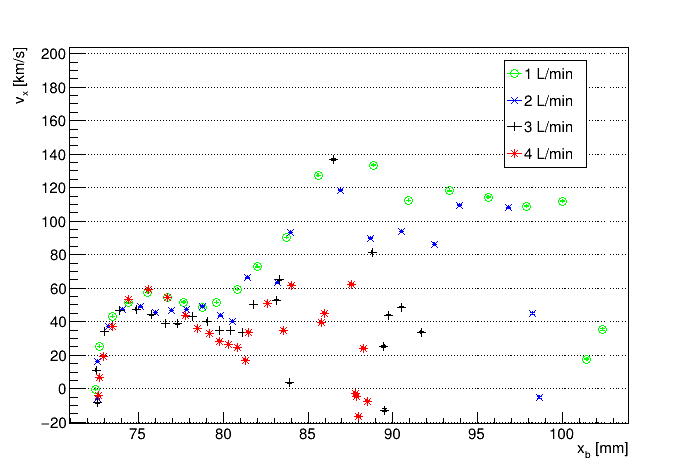
\includegraphics[width=0.48\textwidth]{Images/Shape/elio_035_vx.png}
 }
 \caption{Results of the analysis for different gas flow (opening time of \SI{3.5}{\micro\second} without target).}
 \label{fig:elio_d}
\end{figure}

\begin{table}
 \centering
 \begin{tabular}{ccccccc}
 \toprule
 Flow [L/min]    &$t_{0}$ [ns] &$V_{0}$ [kV]    &$x_{\text{dist}}$ [mm]   &$y_{\text{dist}}$ [mm]   &$v_{\text{disp}}$ [km/s]   &$v_{\text{prop}}$ [km/s]\\
 \midrule
 \num{1}  &\num{121.9}  &\num{5.87(8)}    &\num{30.65(3)} &\num{2.75(1)}  &\num{54.33(10)} &\num{113.97(9)}\\
 \num{2}  &\num{120.9}  &\num{5.71(29)}    &\num{26.08(2)} &\num{1.92(4)}  &\num{46.48(2)} &\num{95.16(6)}\\
 \num{3}  &\num{124.0}  &\num{5.41(27)}    &\num{19.38(1)} &\num{1.84(1)}  &\num{39.88(4)} &\num{40.96(10)}\\
 \num{4}  &\num{121.3}  &\num{5.90(12)}    &\num{22.80(3)} &\num{2.30(1)}  &\num{58.89(14)} &\num{61.94(44)}\\
 \bottomrule
 \end{tabular}
 \caption{Result of the analysis with different gas flows. $t_{0}$ is the bullet formation time, $V_{0}$ the bullet formation tension, $x_{\text{dist}}$ and $y_{\text{dist}}$ are the highest distances reached by the bullet from electrode position, $v_{\text{disp}}$ is the velocity in x direction reached inside the nozzle, $v_{\text{prop}}$ is the velocity of propagation in air in x direction.}
 \label{tab:elio_d}
\end{table}


\subsection{Target influence}
Plasma produced with this source will be applied on biological tissues, so it's fundamental to know how bullet behavior changes with different targets.
We use two target typologies: an insulator, where it's seen charge deposition, and a conductor, that permits to measure the current associated with the bullet.

\subsubsection{Insulator}
An insulator target is not expected to have an effect until the bullet reaches it. An intersting effect is seen after the impact of the bullet with the target, as in figure \ref{fig:elio_ins}, where the plasma seems to deposit charge on the insulator.
\begin{figure}
 \centering
 \subfloat[Bullet propagation \SI{437.6}{\nano\second}.]{
    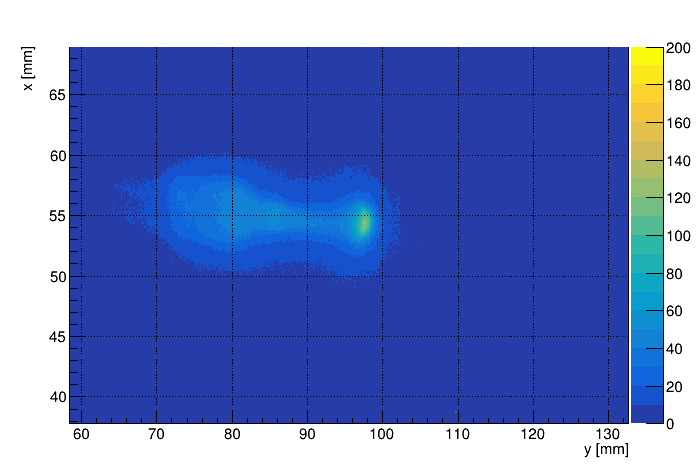
\includegraphics[width=0.32\textwidth]{Images/Shape/elio_ins1.png}
 }
 \hfill
 \subfloat[Bullet impact \SI{457.6}{\nano\second}.]{
    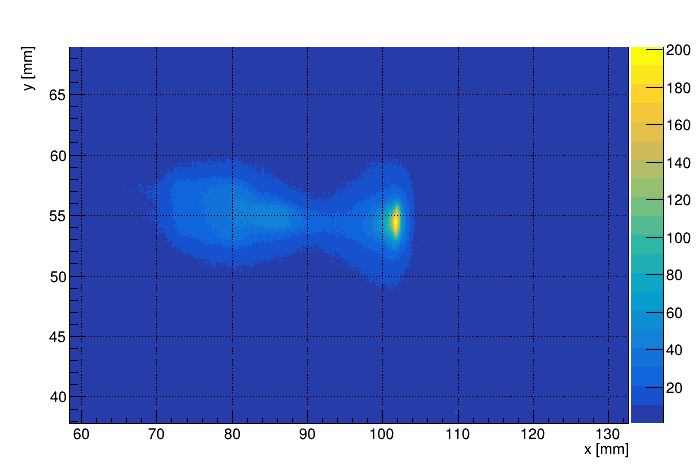
\includegraphics[width=0.32\textwidth]{Images/Shape/elio_ins2.png}
 }
 \hfill
 \subfloat[Charge deposition \SI{577.6}{\nano\second}.]{
    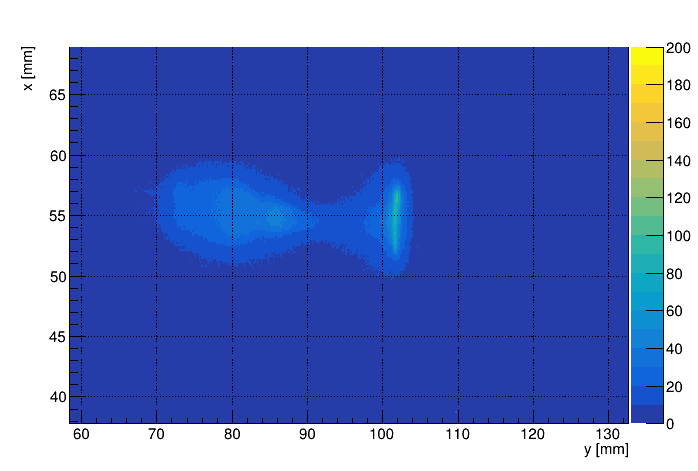
\includegraphics[width=0.32\textwidth]{Images/Shape/elio_ins3.png}
 }
 \caption{Impact time and charge deposition on an insulator target.}
 \label{fig:elio_ins}
\end{figure}


\paragraph{Charge deposition}

\subsubsection{Conductor}
A conductive target is expected to affect bullet behavior as it reachs its proximity, as there are free charges on the surface. If with an insulator we see charge deposition, with a conductor we see a rapid backstream (with a motion inverse to that of the bullet) with great luminosity when the bullet impacts on it, as in figure \ref{fig:elio_met}.
\begin{figure}
 \centering
 \subfloat[Bullet propagation \SI{371.2}{\nano\second}.]{
    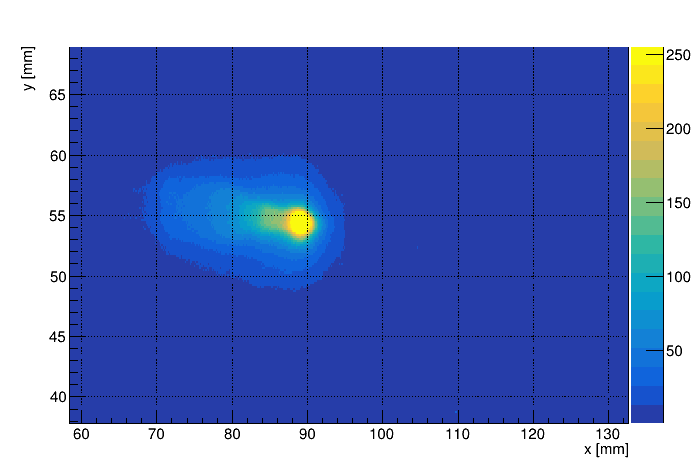
\includegraphics[width=0.32\textwidth]{Images/Shape/elio_met1.png}
 }
 \hfill
 \subfloat[Bullet impact \SI{391.2}{\nano\second}.]{
    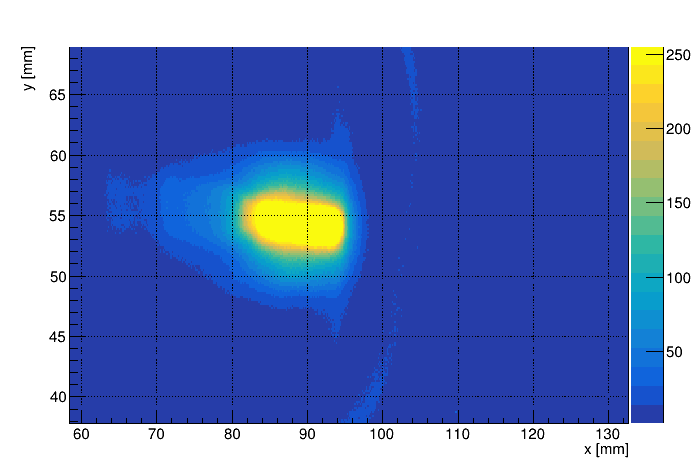
\includegraphics[width=0.32\textwidth]{Images/Shape/elio_met2.png}
 }
 \hfill
 \subfloat[Backstream \SI{411.2}{\nano\second}.]{
    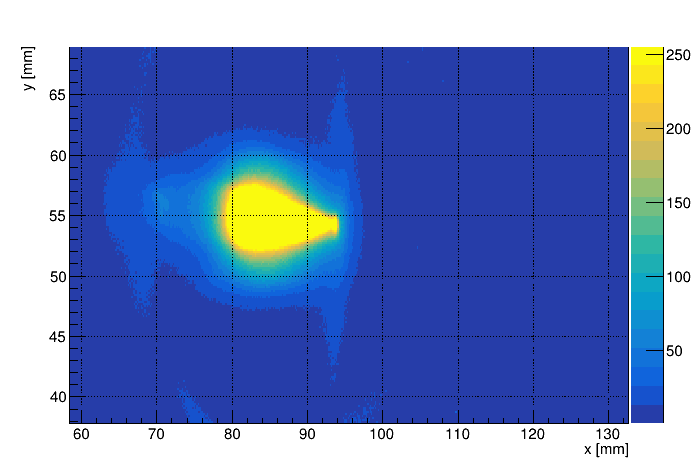
\includegraphics[width=0.32\textwidth]{Images/Shape/elio_met3.png}
 }
 \caption{Impact time and charge deposition on an insulator target.}
 \label{fig:elio_ins}
\end{figure}


\paragraph{Current measure}

\paragraph{Backstream}

\section{Neon flow}
%It's an easy to ignite gas and with high luminosity


\section{Argon flow}
%It's a very hard to ignite gas and with medium luminosity.


%\section{Simple 1D-model}
%General desription, why and Comsol.

%\subsection{Theory}

%\subsection{Results and measure comparision}


%\section{Profilo di temperatura}

%\subsection{Setup termocamera e termocoppia}

%\subsection{Misure di temperatura}
